\documentclass{article}
\usepackage{graphicx} % Required for inserting images
\usepackage{multicol} % For two-column layout
\usepackage{hyperref}
\usepackage[utf8]{inputenc}
\usepackage{csquotes}
\usepackage{float}
\usepackage[margin={2cm,2cm}]{geometry}

% Automated the Figure referencing and make it fully clickable
% \newcommand{\FigRef}[1]{Figure~\ref{#1}}
\newcommand{\FigRef}[1]{\hyperref[#1]{Figure~\ref{#1}}}

\title{
    Virtual machine to container migration system \\(vm2cont)
}
\author{
    Antonio Takev
} 
\date{December 2024}


\begin{document}

\maketitle

% Custom block for affiliations
\begin{center}
    \parbox{0.8\textwidth}{
        \centering
        Master of Applied IT at Fontys University  \& \\ 
        Department of Research and Education at Sue B.V.
    }
\end{center}

% Abstract and Keywords in single-column format
\begin{abstract}
Abstract 
\end{abstract}

\textbf{Keywords:} containerization, black-box migration, dockerization, file system analysis

% Start two-column layout
\begin{multicols}{2}

\section{Introduction}
The software industry is continuously growing and has gone through a natural evolution from native to virtualized, to cloud, and now to container technology, making the term containerization quite popular among developers and companies of all sizes [1]. While containerization is a well-known technique in today's software and cloud-native technologies domain, . The paper is based on the research assignment provided by the Netherlands-based company Sue which specializes in cloud-native technologies, providing a cloud-native platform, managed services, and consultancy in the area of Cloud and DevOps. Working with a variety of big clients such as Dutch Police, Booking.com, Rabobank, and KPN, Sue became a leader in cloud-native solutions. They have built a robust cloud platform called Multistax which hosts applications on Kubernetes clusters. However, around 70\% of their workloads at the moment are still residing in virtual machines. Virtual machines cannot provide a lightweight and easy-to-move interface so that developers can examine what kind of dependencies the application uses and then move the application to another environment in a quick and error-free way. Containers provide a lightweight, user-friendly approach to package an application and all its dependencies and then ship it in any environment while also being able to rapidly transfer it from one environment to another. To modernize its infrastructure and apply containerization, the company aims to automate the process of migrating applications from virtual machines to containers and therefore Kubernetes clusters. As containers offer a more lightweight, isolated, and portable environment, they seem to be the future of cloud deployments. To cover all this, Sue has created the project “Application Profiling” to research how to gather the various dependencies, components, and configurations necessary for the application’s migration from a VM to a containerized environment. During the first iteration of the project, a group of students from the Bachelor’s in ICT and Software Engineering at Fontys University of Applied Sciences developed a tool that could extract and describe the files and packages from a VM and generate a Dockerfile. The tool was built to gather a list of packages, configuration, and application files from a VM and then build a Dockerfile based on them using AI and more specifically ChatGPT. The solution required manual work and was not extensible which made the stakeholders from Sue not so confident in the advantages of using AI to fulfill the project needs. The project goal is to overcome these limitations by automating the generation of an application profile and the creation of a container based on it. While there are some technologies like KubeVirt, Virtlet, and RancherVM which at first glance seem to work on the issue of automated migration, they do not make any migration but provide a way to run VMs in Kubernetes clusters directly (KubeVirt, Virtlet) or package them in Docker images (RancherVM). The only product that provides a tool to make an actual migration is Migrate to Container, offered by Google Cloud. However, this tool works in the close environment of Google and can be used only if the migration of an application from VM to container will be performed within the Google Cloud ecosystem. Considering the lack of tools or systems to migrate applications residing in virtual machines to containers, this research paper takes this as a main research gap. While usually automation issues are considered problems that can be solved through scripts, this research paper aims to go beyond this and research the possibilities of designing an enterprise-level system that can transfer applications from VMs to containers focusing on different topics that have to make the system lifecycle complete. In the paper, several segments of the system will be closely examined as separate but connected topics: Software Architecture design, Software Design patterns, User experience, File system analysis, and Infrastructure management. The research paper aims to design the software architecture and infrastructure of a software system that automates the process of migrating stateless applications from virtual machines to containers so that the applications can be deployed in Kubernetes clusters.

\section{Background}

\subsection{Containerization}
The concept of containerization, as stated in [2], can be found in early 1979 with the introduction of UNIX Version 7 which allowed process isolation by changing the root directory of a process. Containerization is a method for virtualizing programs [3] and the container is a lightweight alternative to VMs to co-host multiple applications on a single server [4]. The shipment of containers-based applications makes them available, tested, and deployed on many servers [3] providing independent plans for upgrades and maintenance [1]. Before containers, developers had to face many challenges when migrating an application from one virtual machine environment to another as usually no two environments are similar in terms of both software and hardware capabilities [1] and it is hard to examine what is running and had been installed on the virtual machine so that it can be replicated in the new environment.
As containerization gained popularity, many companies started migrating from virtual machines to containers for their legacy applications. As stated in [1] using containers results in operational efficiency as containers package the applications with all their required dependencies in terms of software, libraries, configuration files, binaries, and other required data to execute the application. This helps developers run the application in any environment already shipped with all its dependencies [1], and the use of a container benefits both the development and deployment of software [3].

\subsection{Black-box migration}
The transition from VM-based to container-based environments is gaining traction, as containers provide better performance and resource efficiency while still addressing challenges like isolation and dependability [4]. There are several well-known tools to make use of VMs in Kubernetes clusters, examples of which are KubeVirt, Virtlet [9], and RancherVM[10], but this is not the desired goal. The purpose of the project is to design a tool for the migration of an application from a VM to a container and only the Migrate to Containers tool, provided by Google [11] offers a solution for that. As stated in [11], Google Migrate to Containers is a tool designed to convert VM-based workloads into containers within Google Kubernetes Engine (GKE) or GKE Enterprise. This tool supports migrating workloads from on-premises VMware environments or Google Computer Engine [11], while tools like RancherVM provide a solution for packaging and running VMs as Docker containers [10], thus allowing VMs to be managed as if they were containers within Docker. KubeVirt allows the management of applications residing in VMs through Kubernetes by enabling VMs to be run as Kubernetes pods [10]. Virtlet is a similar tool that is not anymore maintained according to their official \href{Github repository}{https://github.com/Mirantis/virtlet}.
Google Migrate to Containers supports the modernization of the following workloads: Linux VM containers, Linux-based workloads (Tomcat, Apache, JBoss, WebSphere, WordPress sites), and Windows IIS applications [10]. Migrate to Containers by Google supports migrations of VMs to containers on Google Kubernetes Engine on the following 64-bit Linux operating systems: CentOS, Debian, RHEL, SUSE, and Ubuntu [10]. The tool supports all Linux-based operating systems for Linux-based workloads [10]. Google Migrate to Containers provides possibilities to migrate VMs to containers on different Linux distributions through a CLI tool that collects the file system [10]. Containers being a packaging unit for any application and producing operating system level virtualization [1], can be viewed as a core principle of achieving system deployments and runtime portability across different operating systems.
In the documentation of Google Migrate to Containers [10], it is stated that they copy the file system of the target machine and perform analysis on this. In this paper this approach will be recalled under the name: "file system analysis" and it can be used to migrate an application from a VM to a container. In Linux, everything is a file [24], allowing such an approach to be able to get the application file, exposed ports, and services used by an application that has to be transferred from a virtual machine environment to a container environment. In all operating systems, there is one abstraction, called process, which can be defined as an "instance of a program in execution" or as "the execution context" of a running program [25] which provides a second option to see what an application is using in terms of application files, exposed ports, and services. The second option will be recalled under the name of process analysis with the same goal of being able to migrate an application from a VM to a container. By briefly introducing both approaches, it can be seen that the first challenge of the research was to collect the essential application information such as application files, ports, and services used by the application through Linux commands which can be performed on a live running VM. Next to this challenge, the core of this research project was built on the goal of migrating an application without knowing what is the application type or technical stack and with just limited user input. In simple words, this can be formulated as black-box migration as the system needs to be designed so that it can perform migrations of applications without or with minimum knowledge of their type, structure, and technical stack. Both file system analysis and process analysis can be used as migration approaches to fulfill the requirements of performing black-box migration.

\begin{figure}[H]
    \centering
    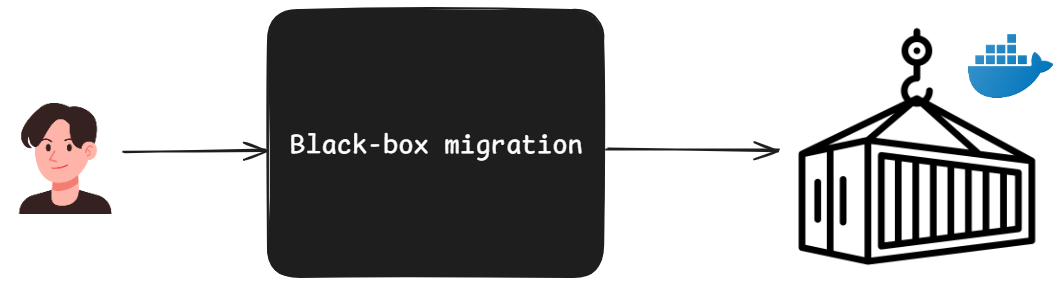
\includegraphics[width=\linewidth]{images/black-box-migration.png}
    \caption{Black-box migration}
    \label{fig:black_box_migration}
\end{figure}

\subsection{Software architecture}
Software architecture plays a main role in providing scalability and maintainability and aligning technical decisions with business objectives [5]. Recent trends emphasize microservices, and cloud-native architectures as key approaches to achieve these goals [5] and modular monolith as an approach that is gaining popularity [6]. As stated in [5], modularity, loose coupling, and high cohesion are some of the best practices to make a scalable and fault-tolerant software system. In the world of enterprise-level software systems, big and small companies tried microservices. As stated by [6] some gain advantages like independent development and deployment of the core units of their software while others do not get the expected benefits and experience issues such as high costs and complexity of the system. As explained in [6], Modular monoliths are organized in well-defined, isolated modules that can be worked independently but deployed as a single unit. The well-known principle of separation of concerns (SoC) can be used to decompose software systems into manageable units [18], particularly useful in the context of a migration system with separation between the CLI interface and core unit managing business logic. Decomposition of the system into units will help achieve ease of change, more localized maintenance, and reuse [18]. Considering the CLI will act as the only point of interaction between the system and the user, the possible options of the core unit are to be developed as part of the CLI or as separate unit, most commonly API. API technologies such as REST, GraphQL, and gRPC further complement modern architectural trends by facilitating efficient communication between distributed systems [7]. While REST remains the most mature and widely adopted API approach, GraphQL and gRPC are increasingly favored for more dynamic, high-performance systems, particularly in real-time applications [7]. This shift towards using the right API for the right use case highlights the importance of aligning technical architecture with both current needs and future scalability requirements [5], [7]. Regarding APIs, REST remains the most mature and widely adopted technology, though GraphQL provides greater efficiency in dynamic, data-intensive applications [7]. gRPC excels in high-performance environments, particularly in real-time applications, as seen in its adoption by companies such as Netflix and Google [7].

\subsection{Design patterns}
Software architecture design is the first step in the process of creating a solid system that corresponds to the user and business needs. Going more in-depth into the solution, people usually try to solve commonly occurring problems that can be solved through the use of design patterns. By definition design patterns are well-known and good solutions to a common problem [21] and provides several benefits such as reusable software, reduced complexity, reduce of the learning time and help novice perform like an expert [22]. Design patterns gained popularity through Object-oriented programming (OOP) and the trend of using various principles and best practices to make the codebase more powerful and future proved. Design patterns vary in its purpose and goals and are commonly organized in the following families: Creational, Structural, and Behavioral [22] and can be used alone or in combination no matter which family they originate from. Creational family abstracts how objects are used by hiding the specifics of the creation process, Behavioral design patterns focus on the relationship between objects or classes, and Structural patterns are used to combine objects and classes into larger structures while keeping them flexible [22]. 

\subsection{User experience}
CLIs are used primarily by humans and usability should be one of the focus points of its design [14], but they are not designed for humans first, nor do they provide a good level of interaction design [13]. The conventions of the UNIX environment such as standard in/out/err, signals, and exit codes ensure different programs work together nicely [13]. Plain, line-based text can be easily piped between commands, while JSON allows integrations with the web [13]. Building the CLI to follow already existing industry patterns, makes the CLI more intuitive [13], [14]. Options should be human-readable and supplemented by short aliases like -v for –verbose [14] but if the user is still unsure how to proceed intuitive help command must be provided [15]. Versioning of the CLI is crucial so that users can easily check if a certain version has a bug report [15]. A long period without output is not user-friendly [15] and the output has to be designed to be human-readable, offering JSON when needed. [12]. As stated in [13], people should be able to search for CLI documentation through a web interface. To design the CLI to be lightweight, [15] advises moving as much business logic as possible out of the actual CLI script and utilizing modular code design. To build a lightweight and user-friendly CLI, a core unit managing the business logic needs to be designed. The core unit needs to collect the application’s data, analyze it, and create a Dockerfile based on it. The collection of the application’s data is particularly important to provide a good user experience. Thus, the usage of agentless tools/scripts to collect application data will be a crucial step towards improved user experience and a more lightweight software architecture. As stated in [11] automation is the way to run tasks without human interventions and the CLI aims to achieve the collection of the application’s data without relying on manual actions from the user such as installing a piece of software on the target VM. Although there are several well-organized blog posts ([12], [13], [14]) on the topic of CLI design, there are no defined design principles or trends described in research papers or whitepapers in command-line interface design or code structure. The only official style guide of a common CLI tool appears to be the Heroku CLI style guide, designed to be human and machine-readable, with strict naming conventions and advice on using colors when outputting [15]. This opens a gap in creating a software architecture style suitable for building lightweight, user-friendly CLIs following comprehensive interface design principles.

\section{Methodology}
To design a software system to migrate an application from a virtual machine to a container a custom Agile-inspired approach with 4 phases was created \FigRef{fig:work_approach} combining DOT framework methods, the Technology Impact Cycle Tool (TICT) for Ethical check, and the Agile mindset. By design, Agile is a way to respond to changes and succeed in an uncertain and turbulent environment and as Agile Manifesot stands [23] the aim is to deliver results frequently promoting reflection on the work at regular intervals of time and maintenance of constant working pace. As in software development, in the academic research domain, the project context, direction, and requirements are continuously changing based on the findings and experiments, which requires a flexible approach with the possibility to back and forth. The approach consists of the following phases: Analysis, Design, Expert review, and Prototype \& Test. The approach is in the form of a cycle of these steps which is completed once the results are satisfying but several iterations of the cycle were made to achieve the desired results.

\begin{figure}[H]
    \centering
    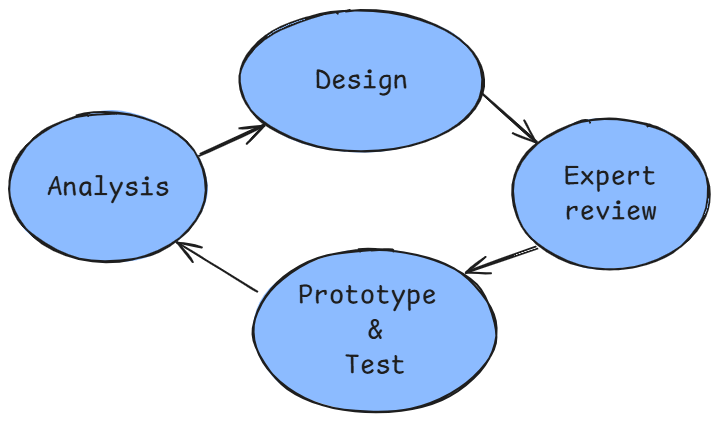
\includegraphics[width=\linewidth]{images/approach.png}
    \caption{Work Approach}
    \label{fig:work_approach}
\end{figure}

The Development Oriented Triangulation (DOT) framework was used to support the ICT research and a core technique of the framework, called triangulation was utilized to combine a mix of research methods to cover different views and aspects of the research. The research methods from the DOT framework are presented in several phases: Library, Field, Lab, Showroom, and Workshop. To research well-known architecture styles, best practices in architecture design, or ideas, rules, and trends for making user-friendly command-line interfaces, Literature review as method from phase Library was used as a method. In addition to literature, Design pattern research from the Library phase was also used to design the system to be extensible and flexible. As the primary goal of the project was designing the architecture of the system, the IT architecture sketching method from the Workshop phase was used to sketch the architecture of the system that can perform black-box migration of an application from VM to container. As a natural result of the design step, the Prototyping method from the phase Workshop was used to build a PoC for showcasing the system component of black-box migration using file system analysis as a migration approach. Finally, a Non-functional test as a method from phase Lab was added to the project to validate the success rate of the system and its usability capabilities.
During the Analysis phase, detailed background research on the topics of Migration strategy, Architecture design, Design patterns, and User experience was conducted. As part of the background research, a list of research papers was closely examined and the gathered data was structured into the following sections: General information, Concepts and Definitions, Research gaps and supporting evidence, Relevant results, and Inspiration. As part of the analysis phase Ethical check was made which makes certain points clear. After the Analysis phase, the next phase is Design which focuses on designing the software architecture of the system with all its components - CLI and core unit managing the business logic. To design the system both Excalidraw and Diagrams.net were used. After the design phase expert reviews were conducted to evaluate the software architecture design and the architecture styles and decisions chosen. In the last phase of the approach, the goal was to create a prototype of the backend API that performs a migration and then test the successful rate of the system. After that the CLI had to be prototyped and the API had to be enhanced to be extensible. Non-functional tests on usability and extensibility had to be performed to check if the system was designed well. The last point of the prototype and test phase is to design and explain the infrastructure strategy for managing the system components.

\subsection{Ethical check}
In terms of human values, the system can replace the manual process of migrating an application from a VM to a container in a more automated way. To achieve this goal Sue employees can be empowered to produce modern deployment strategies for clients that have legacy applications still residing in VMs. This way the company can focus on clients' real desires and "pains". The main stakeholders are the Product owner - Nathan Keyaerts (DevOps Engineer \& Research, Training \& Education Lead at Sue), and Sue's employees they can change the direction of the project and continuously provide both academic and technical feedback but also business-oriented advice. The system is designed for the employees working at Sue and this forms a bias based on their demographics and financial status. Another company might like to take a different approach when solving the issue. Regarding data management the system does not use data collection, it is a way to automate the process of migrating an application from a VM to a container which means that every application is unique and contains real data in this sense. As personal data, GDPR, and privacy are important topics for a system that aims to migrate real applications, a closer look was taken. The technology can register personal data if the application contains a self-contained database or other type of data sources. Most probably this data would be already encrypted. To avoid any GDPR-related issues, the system must be used only by the employees of Sue to automate such migration. If this system is determined useful, then it might be acquired by other companies that have similar issues as Sue. Additionally, it can be designed to serve a bigger amount of users and ideally save a lot of time for big and small companies, allowing the employees to focus on tasks requiring more in-depth work.

\section{Results}
During the analysis phase, knowledge about the context of the project and its topics was gained and terminology and background information were introduced as the base of the research. In the next phase of the research, the system's architecture was created with all the needed components. To generate a solid architecture that is ready to be implemented, it was decided to make several iterations on the design while also working on the technical challenge of building a PoC that performs a black-box migration. The architecture design was created upon more specific requirements without being overcomplicated or unrelated to the project context.

\subsection{Software architecture}
From the start, the system was designed with two components: a command-line interface (CLI) which the user can interact with, and a core unit that handles the business logic. Through the CLI the user can analyze the application profile (application files, ports, services) and create a Dockerfile based on this profile, which will result in a Docker image and container that can be executed alone or as part of a Kubernetes cluster. The core unit acts as a backend which is why it is responsible for handling the user's requests.
During the architecture design phase, several architectures were examined and their advantages and disadvantages were outlined so that in the end one architecture style or a mix can be selected and developed as part of the technical experiment of the research paper.

\subsubsection{Monolithic and N-layer monolithic architecture}
The two main components of the system: CLI and back-end could be placed in one monolithic system \FigRef{fig:monolithic-architecture} which means both the CLI and the back-end will be developed and deployed together. Using this approach the developer is writing the service/business logic directly in the CLI. The approach can be extended by using SOLID principles and SoC and detach the service logic from the CLI by organizing the code base into layers, inspired by the N-layer architecture style \FigRef{fig:n-layer-monolithic-architecture}. The system can be packaged as an all-in-one CLI tool which can be either installed as an executable/binary or accessed through a web interface by the user. In the case of utilizing a monolithic architecture style, the main issue is the future view as the system cannot really be developed or deployed independently, it is difficult to update and maintain it, it will be hard to extend it and there is the risk of making the CLI too heavy so that the users will not be happy and will stop download it and use it. The code for all the system components - analyze and dockerize is placed in the same code base which is a convenient benefit because it makes building a PoC a quick and easy challenge. Additionally, the pure monolithic design of the system allows for organizing the back-end in the form of an automated script that can print logs and messages to the console and improve user interaction.

\begin{figure}[H]
    \centering
    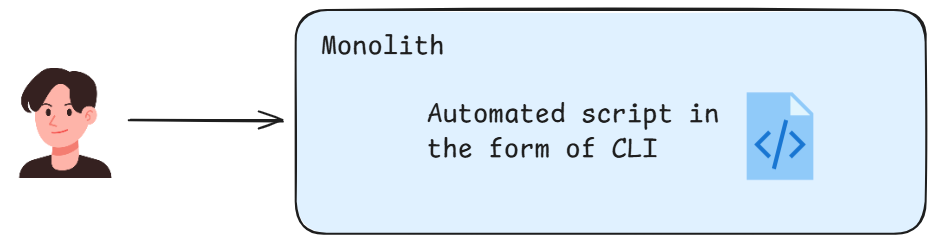
\includegraphics[width=\linewidth]{images/monolithic-architecture.png}
    \caption{Monolithic architecture}
    \label{fig:monolithic-architecture}
\end{figure}

\begin{figure}[H]
    \centering
    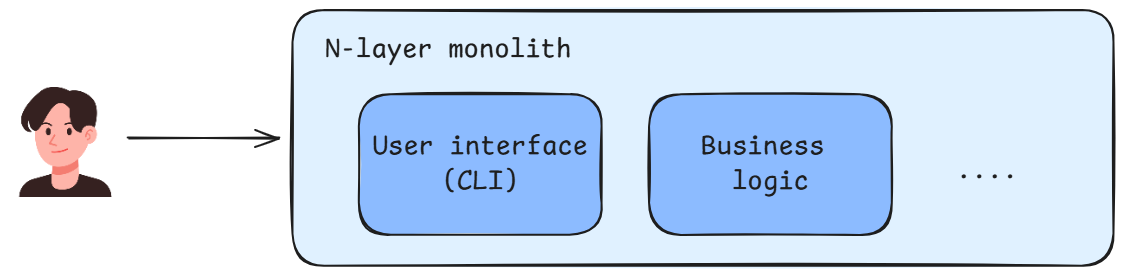
\includegraphics[width=\linewidth]{images/n-layer-architecture.png}
    \caption{N-layer Monolithic architecture}
    \label{fig:n-layer-monolithic-architecture}
\end{figure}

\subsubsection{Headless architecture}
Headless architecture \FigRef{fig:headless-architecture} is a modern style to separate the front-end and the back-end of a website but the same principle can be used to design the migration system as the CLI can act as the front-end and the core unit can be the back-end of the system. In this case, the two layers will be only able to communicate through an API. This adds more flexibility as the developer has the freedom to choose different technology stacks for each layer, but also each layer can scale independently. By separating the layers, the CLI can become much more lightweight, and user-friendly as it will only provide an interface for the user to interact with the system, while the back-end can be deployed on a server on the company's infrastructure or in a cloud environment. This will also improve the performance of the CLI and results in people having to install a CLI tool that is very tiny which increases the likelihood of people using the system more often.

\begin{figure}[H]
    \centering
    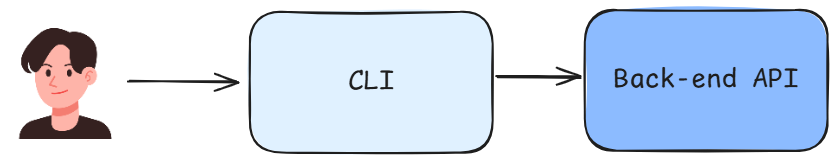
\includegraphics[width=\linewidth]{images/headless-architecture.png}
    \caption{Headless architecture}
    \label{fig:headless-architecture}
\end{figure}

\subsubsection{Headless Microservice architecture}
In today's world microservice architecture style is known as an approach that organizes an application as a collection of two or more services that are independently deployable, loosely coupled, organized around business capabilities, and owned by a small team. In the context of the system, this would mean separating firstly the front-end (CLI) and the back-end and the back-end will be additionally separated into two or more services. For example, the back-end can be organized into Analyze and Dockerize services each responsible for different parts of the migration. In the future, more services could be integrated such as Test service (responsible for testing if the migration was successful through various testing techniques) or Portability service (responsible for investigating the type of OS the application is residing in and add support for not only Linux Ubuntu but also other flavors and even other OS like macOS or Windows). However, this requires each service to be highly detached from the system and makes sense if the system has a lot of service logic or a lot of different components which is not the case for the current state of the system which is more on the PoC level. Another reason for not choosing this style is that it requires more costs to deploy every service and manage it. It will also add complexity in terms of communication between the modules as the middle layer needs to be introduced to synchronize their work and apply messaging. In the context of the project, a combination of Headless and Microservice architecture style is defined so that the CLI and the back-end unit are detached from each other as in the headless architecture and the back-end unit is organized into independent and self-deployable services so that more scalability can be achieved in terms of service logic and routing. All the services communicate with the CLI through a CLI while between each other they can use Messaging solutions like Message Broker (e.g., RabbitMQ, Kafka) to exchange data/information \FigRef{fig:headless-microservice-architecture}.

\begin{figure}[H]
    \centering
    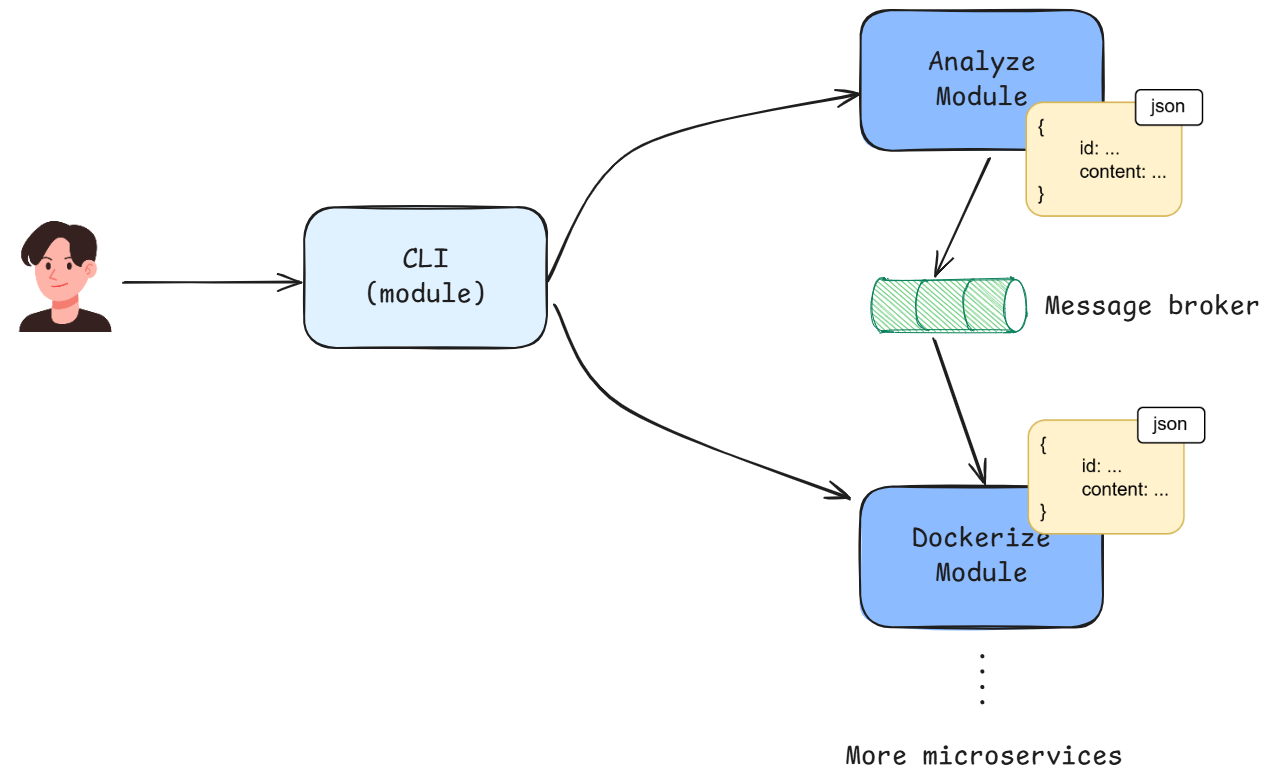
\includegraphics[width=\linewidth]{images/headless-microservice-architecture.png}
    \caption{Headless microservice architecture with microservice-based API}
    \label{fig:headless-microservice-architecture}
\end{figure}

\subsubsection{Headless Modular architecture}
Modular monolith is an approach which combines the advantages of the monolith architecture - simplicity and robustness and the advantages of microservices - flexibility and scalability. This architecture style structures the application into independent modules or components that can be worked alone but deployed together. It promotes both modularity and cohesion of the system. If using this style in combination with the Headless architecture style, everything can be designed as a module - the CLI and all the backend units (Analyze and Dockerize) \FigRef{fig:modular-headless-architecture-level-2}. All the modules can communicate through APIs with the CLI and each module can communicate with each other again through API or as in the Headless Microservice architecture communication between modules can be estabslished through messaging. However, this might be seen as a more complex step in the separation of concerns process which is why a rather simpler design was created which make use of packages instead of modules for the back-end components - Analyze and Dockerize which makes the communication and code organization more beginner-friendly \FigRef{fig:modular-headless-architecture-level-1} and looks like it fits better the current state of project - being a PoC.

And as Martin Fowler said: \begin{quote}
    "You shouldn't start a new project with microservices, even if you're sure your application will be big enough to make it worthwhile."
\end{quote}

\begin{figure}[H]
    \centering
    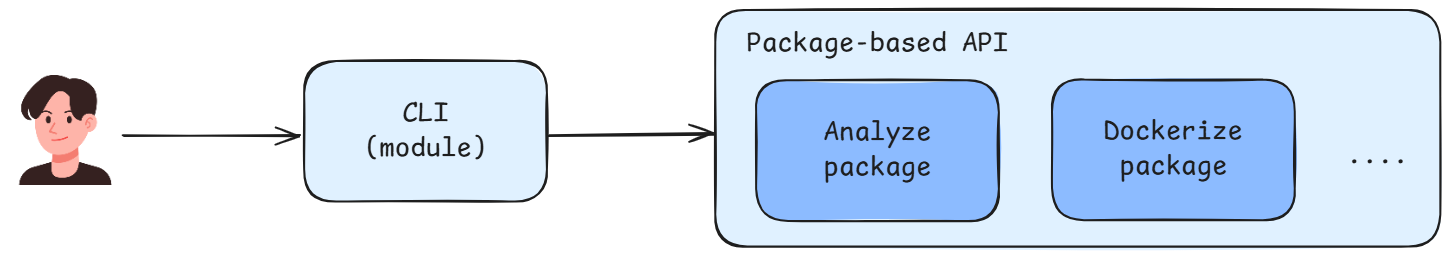
\includegraphics[width=\linewidth]{images/modular-headless-architecture-level-1.png}
    \caption{Modular Headless Architecture with Package-based API}
    \label{fig:modular-headless-architecture-level-1}
\end{figure}

\begin{figure}[H]
    \centering
    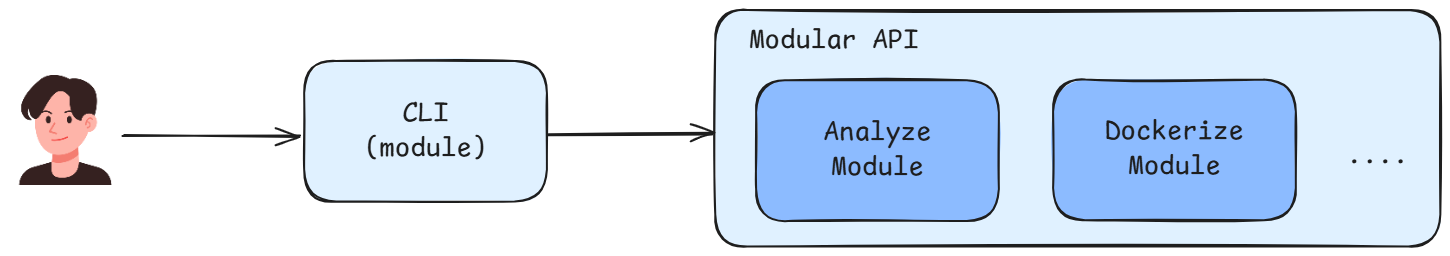
\includegraphics[width=\linewidth]{images/modular-headless-architecture-level-2.png}
    \caption{Modular Headless Architecture with Modoule-based API}
    \label{fig:modular-headless-architecture-level-2}
\end{figure}

\subsubsection{Tech stack}
When choosing the tech stack consultation with the company and the product owner of the project was made which results in several possible options: Golang, Ansible, combination of both or any other technology if it proves to be successful. Ansible is one of the main configuration management tools on the market to automate repetitive tasks and workflows such as configuring network devices, deploying applications, and managing infrastructure [17] and it could be a suitable choice for analyzing the application profile (application files, ports, services). Compared to other tools like Puppet, Salt Stack, and Chef, it is much easier to learn and set up, providing easy-to-read YAML-based syntax [17] that can improve the developer’s experience. As Ansible is designed to be idempotent, running playbooks multiple times will not change the state of the system [17], while Bash/Python/Golang scripts will try to install the same package twice for example. However, Ansible is not a language that can be used to develop a proper API, nor building a system. It is more of an automated tool while Golang can be used for both automation and developing software systems. Golang is also build with the goal to be modular as everything in Golang is a module or package. It is quite lightweight and fast and provides C++-like interface which is appropriate for migration systems where a lot of interaction with the OS interface are needed. To develop the the back-end as an API, the use of the popular framework Gin was made to ease the creation of proper routing. To build the CLI the well-known Golang CLI library Cobra was used to maintain a professional-like CLI tool.

\subsection{Black-box migration}
The core of the technical challenge of the research was in building a PoC for a black-box migration. It was decided to migrate a Nginx web server from an Ubuntu 24.04 Virtual machine deployed on Google Cloud. The PoC was built with idea to be extensible and support more than one migration approaches - file system analysis and process analysis. To make the system flexible, the approaches were designed to be interchangable while also option fo mixed approach was added with the goal to allow user choose if they want certain parts of the analysis process to be taken the file system analysis approach and others by the process analysis approach. The prototype was written in Golang using Gin for building an API interface for the two main interfaces - Analyse and Dockerize. The two components - analyze and dockerize were built as Golang packages to easily communicate to each other and to not overcomplicate the back-end. The prototype successfully performed the migration of a Nginx web server residing in an Ubuntu VM to a Docker container which is run and tested.

\subsection{Design patterns}
Utilizing the Abstract Factory design pattern, the goal was to abstract the concrete implementations of the family of analysis approaches - file system and process from the user and provides a way for the users to choose which approach to use for analysis of their application profiles. The Abstract Factory was implemented with the use of interface that combines all the methods to build the application profile - application files, ports, services and then build a function that acts as a factory entry point with input of the type of the analysis approach and output of the concrete analysis method implementation.
Additionally, the design pattern Strategy was used to make the user even more flexible when choosing analysis apporach by giving opportunity to choose approach for every step of the process, in the current state of the prototype - application files collection, exposed ports collection, services collection. This makes the system be very flexible and user-friendly.

\subsection{User experience}
While user experience was already mentioned in the previous sections, here it will be explained in more details how it was worked out. Firstly, to maintain a lightweight and quickly-to-install interface, the CLI was designed as a binary installable that does not contain any service logic and make request to the back-end through an API interface to gather the results of the analysis and dockerization. The CLI was designed with two main commands - analyze and dockerize. The first command asks for the following input from the user: type (analysis approach type), user (username of the user to access the VM), host (IP of the VM), privateKeyPath (path to the SSH key to access the VM). The dockerize command asks for the following input: dockerImageName (name of the docker image created from the Dockerfile), dockerContainerName (name of the container created from the docker image). Also, output flag was added to provide option for the user to choose between human-readable and machine-readable output, as human-readable output is considered normal text and machine-readable format is considered JSON in the current state of the PoC.

\subsection{Infrastructure management}
As the system was designed to have several components, infrastructure management is an important aspect of the proposed design and prototype. Considering the fact that Sue will need to migrate applications residing in a private network, it is mandatory to have access to this private network to perform any kind of migration. The most straight-forward way of fullfiling this requirement is by deploying the the back-end of the system as a separate module on a self-hosted or cloud-based VM which is part of the private network of Sue. Then the CLI can make requests to the back-end and build a Facade for the user to not know where and how the back-end is deployed and functions. The CLI can be installed from a web interface which is available after providing authentication details which can be gathered on request from Sue's management.

\section{Discussion}
\subsection{Software architecture}
\subsection{File system analysis}
\subsection{Design patterns}
\subsection{User experience}
\subsection{Infrastructure management}

\section{Conclusion}
Summary of the findings and future directions.

\section{Acknowledgments}
Acknowledgments of contributors and funding sources.

\section{References}
\nocite{*}
\bibliographystyle{unsrt}
\bibliography{references}

\section{Appendices}
Additional material supporting the main content.

\end{multicols}

\end{document}

